\documentclass{ntuthesis}

\usepackage{times}
\usepackage{verbatim}
\usepackage{color}
\usepackage{url}
\usepackage{graphicx}
\usepackage{array}
\usepackage{wallpaper} 
\usepackage{amsmath}

% Using the tex-text mapping for ligatures etc.
\defaultfontfeatures{Mapping=tex-text}

% Set the default fonts
\setmainfont{times.ttf}
\setCJKmainfont{kaiu.ttf}

\ifdefined\withwatermark
  \CenterWallPaper{0.174}{./watermark.pdf}
  \setlength{\wpXoffset}{6.1725cm}
  \setlength{\wpYoffset}{10.5225cm}
\fi

% Your information goes here
% author: Tz-Huan Huang [http://www.csie.ntu.edu.tw/~tzhuan]

% ----------------------------------------------------------------------------
% "THE CHOCOLATE-WARE LICENSE":
% Tz-Huan Huang wrote this file. As long as you retain this notice you
% can do whatever you want with this stuff. If we meet some day, and you think
% this stuff is worth it, you can buy me a chocolate in return Tz-Huan Huang
% ----------------------------------------------------------------------------

% Syntax: \var{English}{Chinese}
\university{National Taiwan University}{國立臺灣大學}
\college{College of Electrical Engineering and Computer Science}{電機資訊學院}
\institute{Graduate Institute of Communication}{電信工程學研究所}
\title{Performance Analysis of IEEE 802.11ax OFDMA-based Random Access}{802.11ax 基於OFDMA隨機接取效能分析}
\author{Yang Hang}{楊行}
\studentid{R03942126}
\advisor{Kwang-Cheng Chen, Ph.D.}{陳光禎 博士}
\defenseyear{2016}{105}
\defensemonth{December}{12}
\defenseday{19}


\begin{document}
\AddToShipoutPictureBG{\put(\LenToUnit{.325\paperwidth},\LenToUnit{.35\paperheight}){
\includegraphics[scale=1]{watermark.pdf}}}

\frontmatter

\makecover

\makecertification

\input{acknowledgements}
\begin{abstractzh}
近年來wifi成為分布最為廣泛的WLAN,wifi配置地越來越多,越來越密集,也有越來越多的設備接入wifi,通過wifi的流量也越來越大。
漸漸地,傳統802.11 接取層(MAC)基於分布式競爭接入(DCF)的方式本身的問題越來越凸顯出來,主要表現為碰撞加劇,從而網路吞吐量降低,接入時延變大,能耗嚴重。
我們稱之為密集分布場景(dense deployment scenario)的問題,所以IEEE 802.11成立ax工作組針對密集分布場景的問題,在傳統802.11 接取層(MAC)和物理層(PHY)都進行很大的修改。引入了OFDMA,實現多用戶信道(MU)。
802.11ax提出基於OFDMA的隨機接取,它比傳統的隨機接取更加覆雜,更有彈性。
本論文旨在分析該機制的效能,建立二維離散時間馬爾可夫模型很好地描述了其穩定狀態行為。
並且借此模型分析重要系統參數對系統效能的影響從而得出配置參數的方法。

\noindent
關鍵詞:802.11ax,多用戶信道,OFDMA,隨機接取
\end{abstractzh}

\begin{abstracten}
In recent years, WiFi has been the most extensively deployed WLAN. 
With more and more deployment, devices or users, and exploding traffic, the WLAN is more and more dense. 
Gradually, problem from the nature of distributed coordination function (DCF), which is the foundation of legacy 802.11 MAC, has arisen and is becoming more and more severe. 
That is, severe collision causes degradation of throughput, defer access, and waste energy of stations, which in total is called dense deployment problem. 
Thus, task group IEEE 802.11ax, which was set up in 2014 confronting the above problem, makes revolutional modification of both MAC and PHY to legacy 802.11. 
OFDMA is issued in 802.11ax, implementing Multi-User (MU) channel. 
And correspondingly, 802.11ax proposes OFDMA-based random access, which is more complicated and flexible than legacy random access. 
This work model the OFDMA-based random access with bi-dimensional discrete-time Markov Chain to accurately depict its steady state behavior. 
With this model, we evaluate the effect of several system parameters and propose rules of configuring the parameters.



\noindent
\textbf{Keyword: 802.11ax, MU PHY, OFDMA, random access}
\end{abstracten}

\begin{comment}
\category{I2.10}{Computing Methodologies}{Artificial Intelligence --
Vision and Scene Understanding} \category{H5.3}{Information
Systems}{Information Interfaces and Presentation (HCI) -- Web-based
Interaction.}

\terms{Design, Human factors, Performance.}

\keywords{802.11ax, MU PHY, OFDMA, random access}
\end{comment}


\tableofcontents
\listoffigures
\listoftables

\mainmatter

% Your thesis goes here
\chapter{Introduction}
\label{c:intro}

%1. why 802.11ax, dense, DCF, contention, collision
During last decades, IEEE 802.11 achieved great success in WLAN. Enormous WiFi are deployed for its high speed and simplicity of deployment. 
The foundation of 802.11 MAC, distributed coordination function (DCF), is a random access mechanism \cite{bianchi2000performance}.
With DCF, a random access MAC, the star topology of a 802.11 WLAN result in a absolutely unfair queueing. 
Since in star topology,  access point (AP) needs to transmit all the down-link (DL) traffic, which is often more than $1/2$ traffic loading of the basic service set (BSS), while AP has only $1/n$ chance to access medium where $n$ is number of total stations including AP. It is, thus, an unfair queueing problem.
What's worse, combining effect of the unstability of random access's nature and the unfair queueing problem, once under a dense scenario, the performance will degrade severely since contention and collision will occupy the channel.
That lies the defect of legacy 802.11.
We collectively call them dense deployment problem.
The dense deployment problem not only degrades throughput but also waste much energy.

%2. ax feature, MU, central control, but OFDMA-random access
Previous amendments, 802.11n and 802.11ac called high throughput (HT) and very high throughput (VHT) respectively which are aimed at improving throughput, only mitigate the dense deployment problem. 
The bottleneck at the MAC efficiency is not resolved.
Thus, 802.11ax task group is issued targeted at high efficiency WLAN (HEW), improving quality of experience (QoE) and power save.
Confronting the dense deployment problem, 802.11ax permits AP of central control, to schedule both down-link (DL) and up-link (UL) transmission so that contention is much reduced and unfair queueing problem could be resolved.
IEEE 802.11ax also issues multi-user (MU) PHY which is supported with Orthogonal Frequency Multiple Access (OFDMA), and a special control frame called trigger frame (TF) to implement trigger-based MU UL\cite{draft_ax}. %\cite{dengquality}
Accordingly, multi-channel random access, the focus of this paper, is of course implemented in 802.11ax, named OFDMA-based random access, since random access is an efficient way for stations to transmit bandwidth request, buffer status report (BSR) etc. 
Actually, the new MAC is based on DCF since it helps co-exist among BSS and other systems. The difference is that the DCF mainly works on AP which means AP needs to access channel following DCF procedure, while HE-STA (802.11ax STA) is mostly scheduled by AP and even the random access procedure is initialized by AP. 

%3. related work, random acces history ? , clarify OFDMA-based random access is special
% SU/MU; aloha/CSMA; BEB/UB; saturated/unsaturated
Random access is a classical topic in data network which has evolved multiple variants with various physical layer.
Random access originates from Aloha and slotted Aloha in single-user channel. Then CSMA works as typical collision resolution  \cite{kleinrock1975packet}, which is accepted by IEEE 802.11 named CSMA/CA. 
The backoff mechanism, which is about retransmission when failure occurs, is also important in random access.
Random access has been a popular approach to MAC on unlicensed band for a long time, while cellular network  only implements random access for initial up-link access. 
With OFDMA, i.e., MU channel, randomness extends from time domain to frequency domain, 2-dimension. In cellular network, IEEE 802.16 and 3GPP LTE use a multi-channel slotted Aloha.
In the literature, plenty of works focus on the multi-channel random access, and most of them work on cellular network.
\cite{choi2006multichannel} designs a 1-persistent type retransmission, i.e., no exponential backoff, to achieve a fast access.  
In \cite{zhou2008efficient}, a closed-form expression of throughput for OFDMA system is firstly given.
Many works compare performance of two backoff mechanism, binary exponential backoff and uniform backoff  \cite{zhou2008efficient} \cite{seo2011design} \cite{kim2012performance}, which are implemented by IEEE 802.16 and 3GPP LTE respectively.  \cite{wei2015modeling} specifies a model estimating transient behavior of OFDMA system.
%many metrics: throughput, mean and variance of access delay, stability
All above works about OFDMA random access is an Aloha-type access in cellular network.
In addition, \cite{GeneralizedOFDMACSMACA} is one of a few works for 802.11. It generalizes CSMA/CA to OFDMA system for 802.11.

%4. our work
% the first to analyze the 802.11ax random access
Though OFDMA and multi-channel random access have been employed by IEEE 802.16 and 3GPP LTE for a long time.
It is the first time for 802.11ax to issue OFDMA and OFDMA-based random access, which is a huge evolution for 802.11.
And as far as we know, this is the first paper analyzing IEEE 802.11ax OFDMA-based random access. 
It employs binary exponential backoff and MU PHY under Trigger-based MU UL, which is different from \cite{GeneralizedOFDMACSMACA}.
Since \cite{bianchi2000performance} proposes an accurate Markov chain model for DCF, we could also reuse this model to generate another Markov chain for 802.11ax to precisely depict the OFDMA-based random access.
We assume stations are under saturated condition which means they always have packets to transmit.
The saturated analysis is based on the key assumption of independent collision probability $p$ whatever the packet is retransmitted or not.
Simulation validates our model to be accurate.
Then, we estimate the maximum system efficiency and minimum access delay. 
Since OFDMA-based random access has dynamic and more complicated parameter sets than legacy 802.11, we evaluate effect of a variety of parameter sets and at last propose rules for AP to configure the parameter set. 

The paper is organized as follows.
More explanations of 802.11ax features are given in section \ref{sec_ax_feature}. 
In section \ref{sec_RA_illu}, a detailed illustration of OFDMA-based random access procedure is presented.
Section \ref{sec_sys_model} contains the system model and performance analysis, including system efficiency and access delay, of the random access mechanism. 
Then section \ref{sec_model_val} shows simulation results compared with analysis results, which validates the model.
In section \ref{sec_max_min}, additional considerations on optimal performance are carried out. 
Section \ref{sec_perf_eval} gives performance evaluation under various parameter sets and at last propose rules for configuring the parameter set.
Conclusion remark is given in section \ref{sec_conclu}.

%\begin{figure}
%\centering
%\includegraphics[width=0.45\textwidth]{kl}
%\caption{kl-distance}
%\label{kl}
%\end{figure}
%
%\begin{table}[t]
%\begin{center}
%\begin{tabular}{lcc}
%
%\hline
%                    &  {\small Itti's method}     & {\small Fuzzy growing}    \\
%\hline
%{\small Precision}           &  0.4475    & 0.4506 \\
%{\small Recall}              &  0.5515    & 0.5542 \\
%\hline
%
%\end{tabular}
%\caption[Evaluation of FOA sets]{\small Evaluation of FOA sets. } \label{t:FOA}
%\end{center}
%\end{table}

\chapter{802.11ax Features}			\label{chp_ax_feature}
The legacy random access is called distributed coordination function (DCF). 
Since the DCF degrades performance severely at dense scenario solution, IEEE 802.11ax proposes a centralized coordination MAC, improving the status of AP. 
This centralized coordination function is also based on DCF so that 802.11ax is compatible with legacy 802.11 and other wireless system. 
At the same time, multi-user (MU) PHY is issued in IEEE 802.11ax to improve the system performance\cite{dengquality}. 
In this chapter, we first introduce 802.11ax feature, MU PHY, then illustrate the OFDMA-based random access mechanism.
\section{Multi-User PHY} \label{sec_MU}
\subsection{PHY}
While legacy 802.11 specifies a 20 MHz channel a Single User (SU) channel, which means only one user could access the channel at a time in a BSS, 802.11ax issues a MU PHY with OFDMA, allowing multiple STAs to access channel simultaneously.
It should help mitigate contention and collision. 

The channel in 802.11ax is more fine-grained, defined as resource unit (RU) in figure \ref{fig_RU_spec}. 
The smallest RU is 26-tone, with which a legacy 20 MHz channel could be separated into 9 subchannels.
It is flexible that if there are not 9 HE-STAs to share the channel, AP could allocate multiple RUs to one HE-STA without wasting the RUs.
And as specified in figure \ref{fig_RU_spec}, multiple 20 MHz channels can be aggregated to be utilized by a BSS, which is called \textit{Channel Bonding}. 
This will help a lot improve system performance, since one BSS is not restricted to a single 20 MHz channel.  
It is worth mentioning that every transmission of MU should end at the same time. That means padding is required for short packets.



Actually, DL MU PHY has been implemented in 802.11n and 802.11ac with MU-MIMO, which is an absolutely different method from OFDMA and beyond the scope of this paper. 

\begin{figure}[!t]
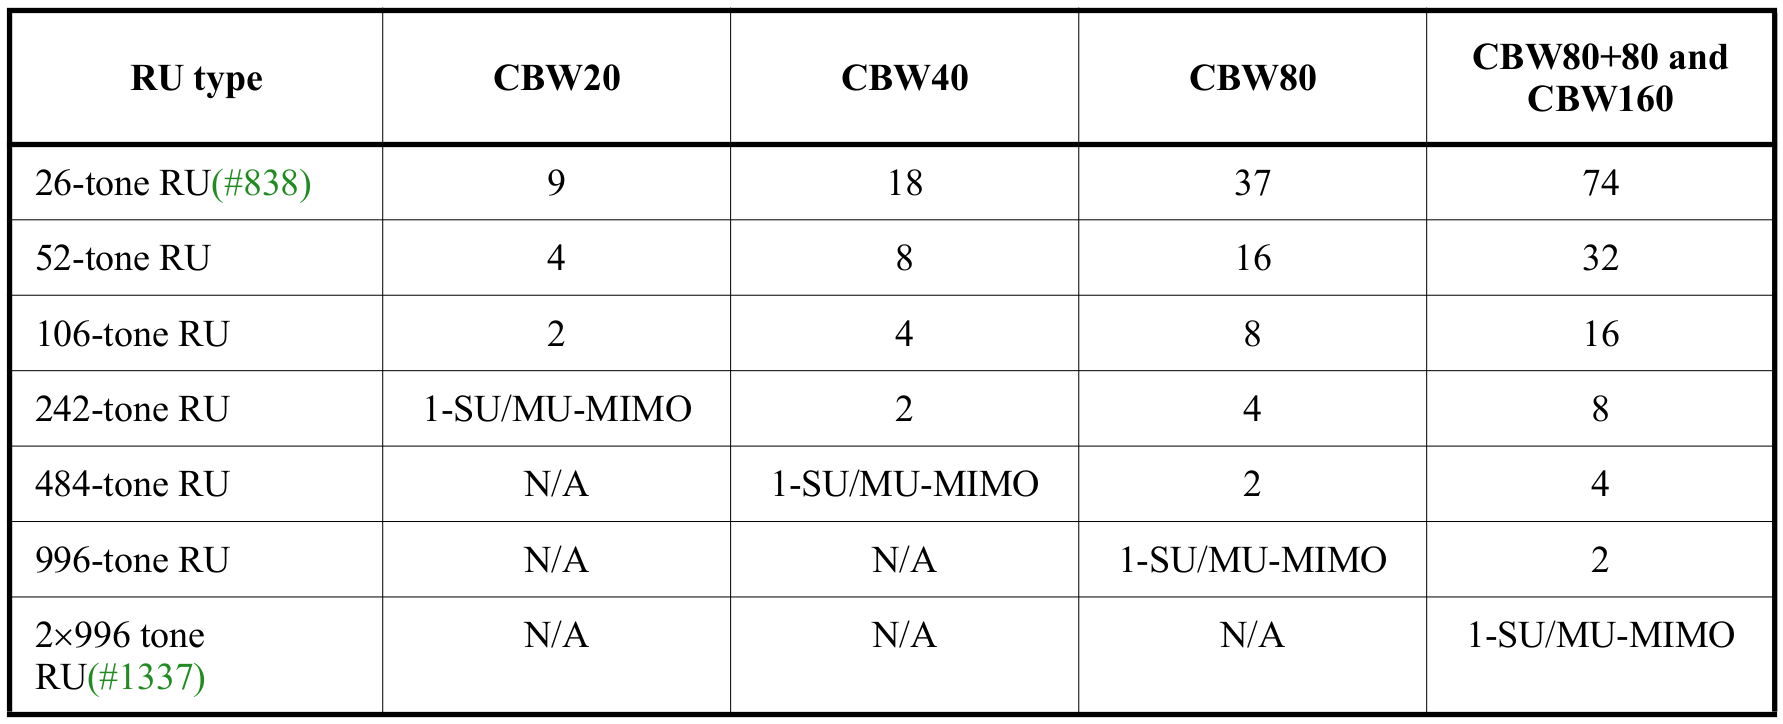
\includegraphics[scale=0.25]{./figure/chp2/RU_spec.png}
\caption{Maximum number of RUs for each channel width}
\label{fig_RU_spec}
\end{figure}


\begin{figure}[!t]
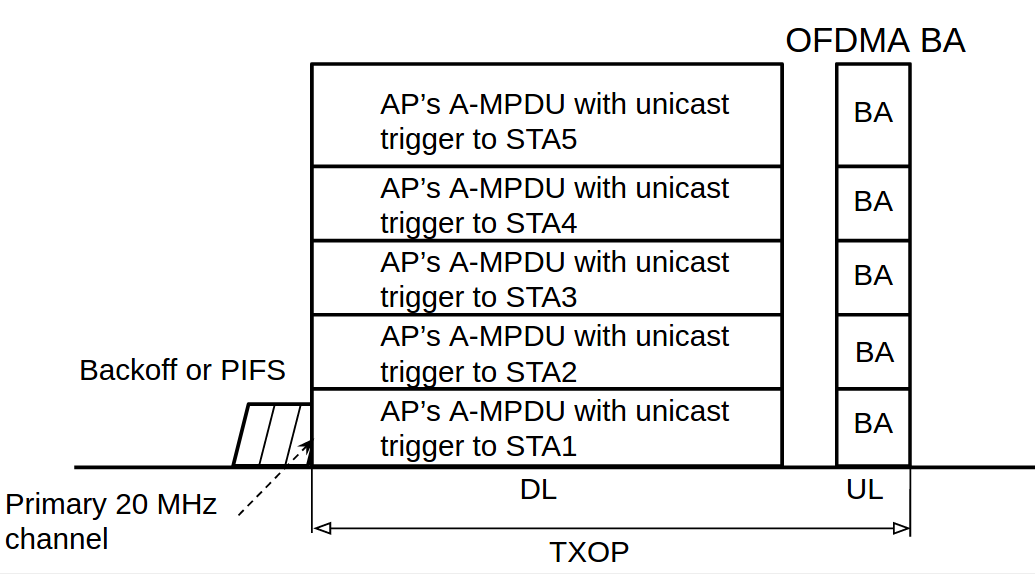
\includegraphics[scale=0.4]{./figure/chp2/fig_MU_DL.png}
\caption{MU DL of 802.11ax}
\label{fig_MU_DL}
\end{figure}


\begin{figure}[!t]
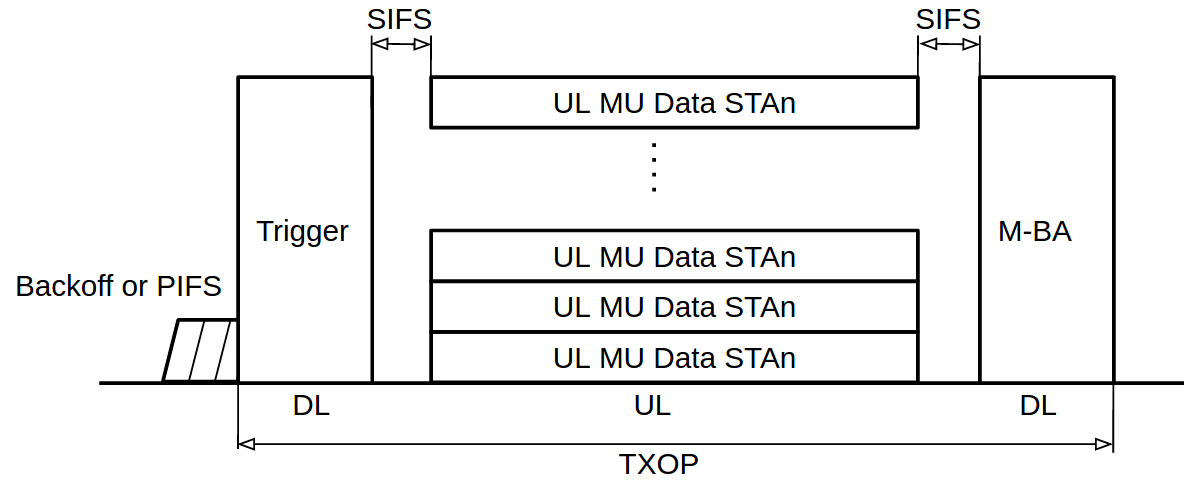
\includegraphics[scale=0.36]{./figure/chp2/fig_MU_UL.png}
\caption{Trigger-based MU UL of 802.11ax}
\label{fig_MU_UL}
\end{figure}


\subsection{MAC}
802.11ax MAC is still based on DCF. However, only AP follows DCF. HE-STAs are scheduled by AP.
AP will contend with DCF procedure to transmit DL packets with OFDMA to multiple stations, which is called MU DL as in figure \ref{fig_MU_DL}. 
The difficulty of OFDMA MU is MU UL. 
802.11 is not a synchronous system, preamble and even two-way handshaking are required before a data transmission. 
A trigger-based MU UL is issued as in figure \ref{fig_MU_UL}.
A brand new control frame, called trigger frame, is created to be transmitted by AP before HE-STAs transmitting a UL packet. 
In this way, stations are able to access channel with RU scheduled by trigger frame transmitted by AP. 
The trigger frame format is as figure \ref{fig_TF_format}. Since the standard is in progress, many fields remain to be determined (TBD). 

\begin{figure}[!ht]
\centering
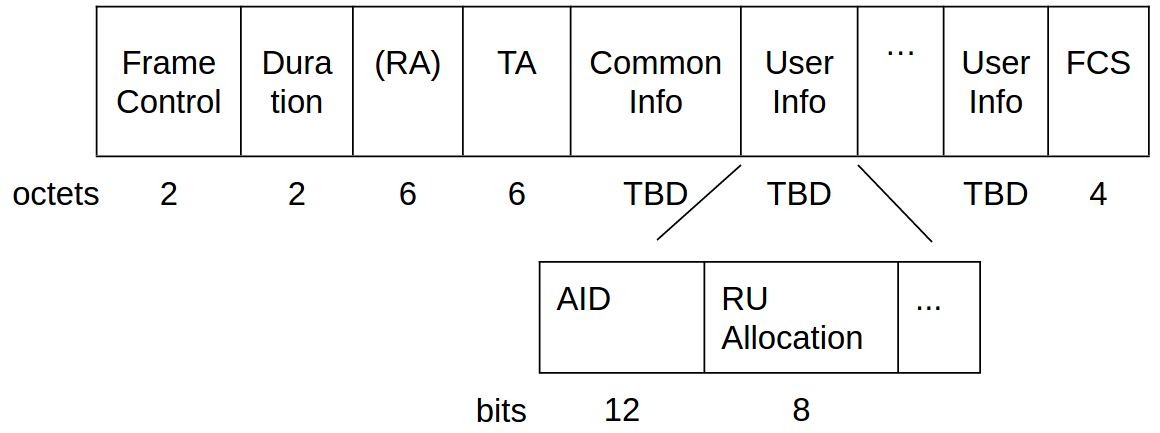
\includegraphics[scale=0.3]{./figure/chp2/fig_tf_format.png}
\caption{Trigger Frame format}
\label{fig_TF_format}
\end{figure}

The basic use of trigger frame is to allocate RUs. It contains resource allocation information in field \textit{user info}, specifying some station to access some RU in subfield \textit{AID} and \textit{RU allocation}.  
When AP schedules RUs for random access, the subfield \textit{AID} of User Info is set to value 0. The detailed procedure we will illustrate in section \ref{sec_RA_illu}. 

What's more, to support scheduling of TF, a mechanism called \textit{Target Wake Time} (TWT) is implemented in 802.11ax. TWT is originally issued in 802.11ah for power saving\cite{khorov2015survey}. It is also out of scope of this thesis.



\section{802.11ax Random Access Illustration}		\label{sec_RA_illu}
\begin{figure*}[!t]
%\begin{minipage}{.5\textwidth}
\centering
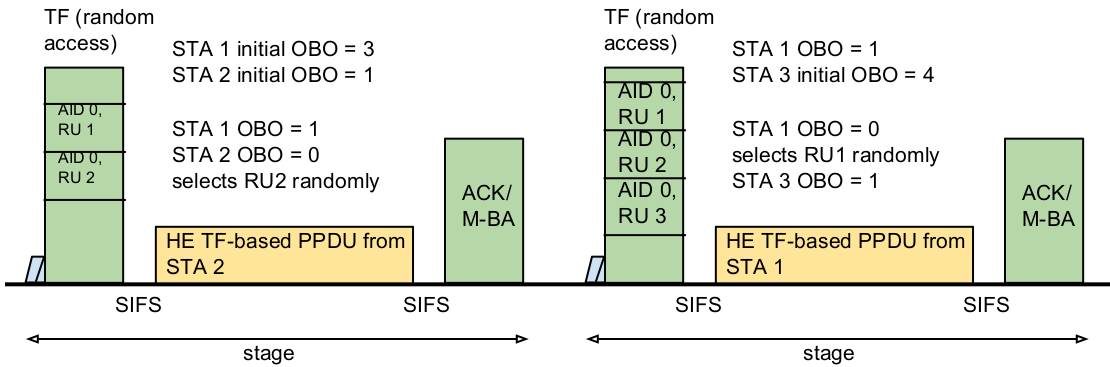
\includegraphics[scale=0.35]{./figure/chp2/RA_illu.png}
\caption{Illustration of OFDMA-based random access}
\label{fig_ra_illu}
%\end{minipage}
\end{figure*}

%\begin{minipage}{.5\textwidth}
%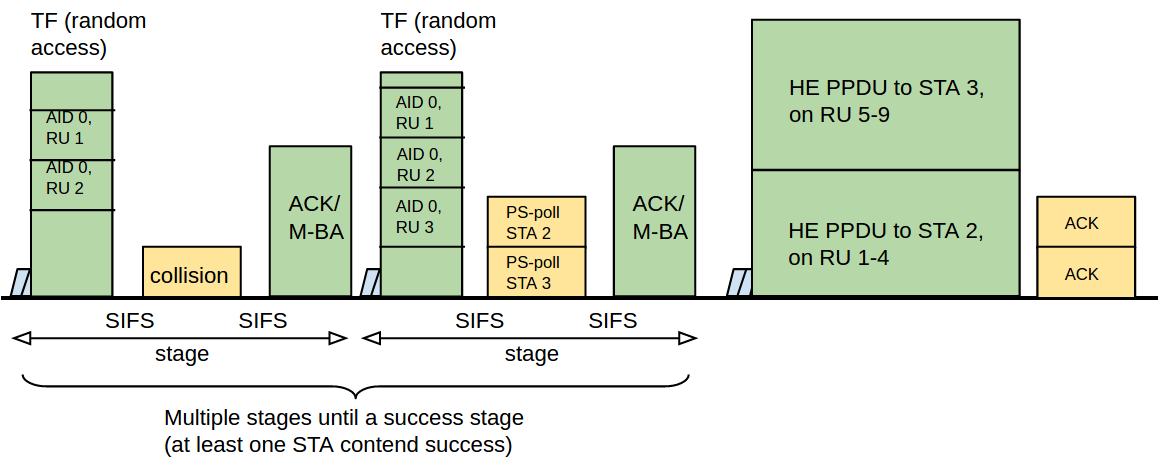
\includegraphics[scale=0.35]{./figure/RA_illu_3.png}
%\caption{Another example of OFDMA-based random access for DL in 802.11ax}
%\label{fig_ra_dl}
%\end{minipage}


\begin{figure}[!t]
\centering
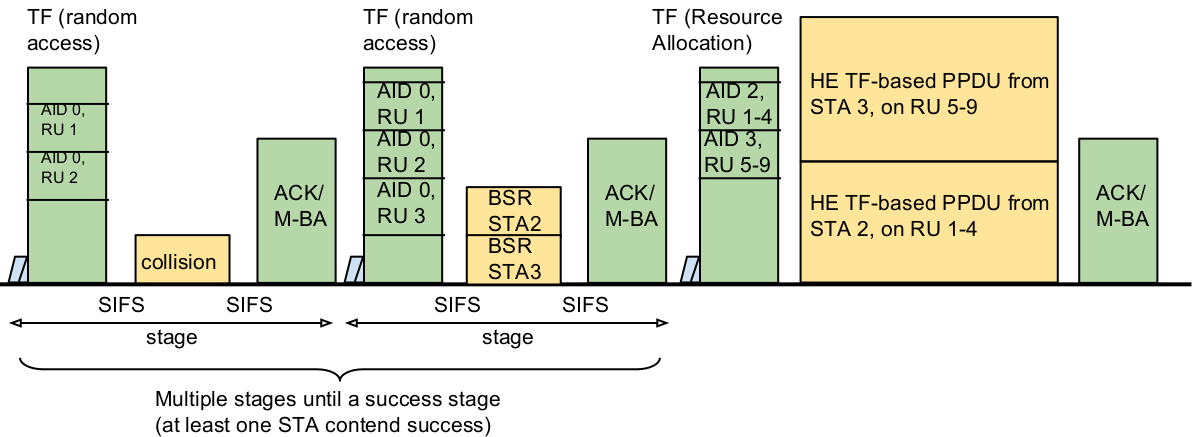
\includegraphics[scale=0.35]{./figure/chp2/RA_illu_2.png}
\caption{An example of OFDMA-based random access for UL in 802.11ax}
\label{fig_ra_ul}
\end{figure}

As stated above, legacy IEEE 802.11 MAC is a 20 MHz SU PHY, which means that at most single user could succeed in contending at a time slot.
With the MU PHY, HE-STA (802.11ax, high efficient station) has multiple RUs to access, which means multiple HE-STAs may access channel at the same time.
And the system parameters are set by AP dynamically.
The procedure is of course more complicated and flexible.
We first illustrate the OFDMA-based random access procedure then give one use case of the random access.

Different from legacy 802.11 where parameters like contention window are pre-set at hardware of station, all the parameters are configured by AP in 802.11ax. 
The parameter set is composed of $OCW_{min}, OCW_{max}, M$. $OCW_{min}$, (i.e., OFDMA contention window), represents the minimum contention window, while $OCW_{max}$ represents the maximum contention window. 
And $M$ is the number of RUs for random access. $OCW_{min}, OCW_{max}$ are given in an element called RAPS (random access parameter set) contained in beacon frame sent by AP.
In this way, HE-STA is able to access channel with different parameters obtained from the beacon frame. 


In a beacon interval, to initialize a random access procedure, AP first transmits a trigger frame. 
The TF announces some RUs for random access by setting the AID of those RUs value of 0. 
HE-STAs need to maintain a backoff counter, called OFDMA Backoff (OBO). 
HE-STAs who want to access channel will randomly generate a OBO among range $[0, OCW_i]$, where $i$ is the backoff level and $OCW$ is retrieved from RAPS sent by AP. 
Then the OBO subtracts $M$, the value of number of RUs for random access in the current stage. 
If the OBO reaches 0, the HE-STA will randomly select a RU from those RUs for random access to transmit a packet after SIFS (short inter-frame spacing). 
After that AP responds with a block ACK indicating who succeed in contending.
The OFDMA-based random access is a three-way handshake, which is totally called a stage. 
It is worth reminding that the stage in this thesis is a concept of interval\cite{draft_ax}, not the backoff stage in papers\cite{bianchi2000performance}. 
To distinguish the two words, we use backoff level replacing backoff stage. 
Those whose OBO is greater than 0 will freeze the OBO and wait for next stage.  
If more than one HE-STA transmit at the same RU, collision occurs. 
Those who collide in the current stage will double their $OCW$ at next stage until $OCW$ reaches $OCW_{max}$. 
Only if at least one HE-STA succeed in transmit a request in a stage will the stage be a successful stage. 

Figure \ref{fig_ra_illu} illustrates the procedure. Green means transmission from AP to STA (i.e., DL) and yellow means UL direction. 
With clear illustration above, we look deeply into the implementation of the mechanism.
See figure \ref{fig_RAPS}, the two critical parameters $OCW_{min},OCW_{max}$ are specified in field OCW Range. 
The value is defined by $OCW_{min} = 2^{EOCW_{min}}-1$, $OCW_{max} = 2^{EOCW_{max}}-1$. 
In the following analysis, we issue another parameter $m$ so that maximum backoff level, $OCW_{max} = (OCW_{min}+1)*2^m-1$. So we specify $OCW_{max}$ with $m$ and $OCW_{min}$ in following section, which simplifies analysis.


Following is a use case of OFDMA-based random access as figure \ref{fig_ra_ul}. 
When HE-STAs want to random access to transmit data packets, he will send buffer state report (BSR) frame with OFDMA-based random access. 
After successful contention, AP will allocate RUs for the HE-STA by trigger frame.
Then stations transmit UL data packets with the allocated RUs. 


Other use cases could borrow the same random access procedure. 
Similar to legacy 802.11 power save, HE-STA needs to transmit PS-poll or APSD-trigger frame to inform AP of its active state when the HE-STA wakes up.
The transmission of PS-poll or APSD-trigger frame is a good case of OFDMA-based random access. After successful contention, AP will transmit the buffered packets of the HE-STA.

\begin{figure}[!h]
\centering
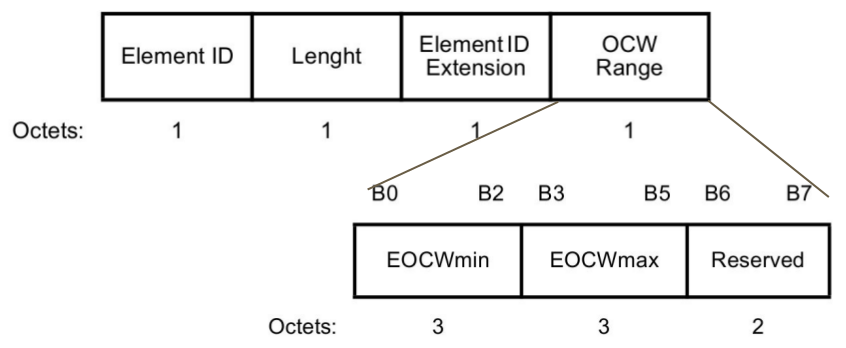
\includegraphics[scale=0.4]{./figure/chp2/RAPS.png}
\caption{Random Access Parameter Set (RAPS) Element}
\label{fig_RAPS}
\end{figure}


\chapter{System Model} 		\label{sec_sys_model}
One of main contribution of this paper is the analytical evaluation of the saturation analysis of 802.11ax OFDMA-based random access, in the assumption of ideal channel conditions (i.e., no hidden terminals and capture). 
The Markov chain model of random access was first proposed by Bianchi for analyzing distributed coordination function\cite{bianchi2000performance}. 
Here, for the brand new ODFMA-based random access, we generate a new Markov chain model. 
In this analysis, we also generate three metrics, $n_s$ number of stations who succeed in contending in a stage, \textit{eff} self-defined system efficiency, and $D$ access delay of request frame. 

The analysis is divided into two parts. First is the Markov chain model to estimate the packet transmission probability $\tau$ and conditional collision probability $p$. 
Secondly, we express the three metrics as function of $\tau$. 
Table \ref{table_notation} is a list of all parameters and notations.

\begin{table}[!h]
\caption{Parameters and Notations}
\centering
\label{table_notation}
\begin{tabular}{c|l}
\hline
$n$						& $\#$ of stations \\
$OCW_{min}$ or $W_0$		& minimum OFDMA contention window \\
$M$						& $\#$ of RUs for random access \\
$m$						& maximum backoff level \\
$p$						& packet collision probability \\
$\tau$					& station's transmission probability \\
$n_s$					& $\#$ of successful stations in a stage \\
$N_{s\_station}$			& $\#$ of stages for a station to succeed in contending \\
$N_{s\_stage}$			& $\#$ of stages until a successful stage \\
\hline
\end{tabular}
\end{table}

\section{Packet Transmission Probability}
Since 802.11ax implements OFDMA-MU and corresponding trigger-based UL, AP won't contend with 802.11ax stations under this situation.
To estimate the performance of the OFDMA-based random access mechanism, we assume a saturated condition that each station always has packets to transmit as long as it accesses the channel.
In the first use case, each station will contend to send \textit{Buffer Status Report} (BSR), for convenience and easy understanding we call it request in the following context, for the data transmission later. 

With above illustration of OFDMA-based random access mechanism, a 20 MHz channel, which is a single user (SU) channel in legacy 802.11, can be divided into 9 subchannels, called resource unit (RU). Consider a fixed number $n$ of contending stations. 
$M$ represents the number of RU for random access in a stage. 
$W_i$ is the OFDMA contention window (OCW) at $i^{th}$ backoff level, with relationship $W_i = 2W_{i-1}+1$. Stations with OCW $W_i$ will randomly generate a backoff counter among range $[0,W_i]$.  

The bidimensional process $\lbrace s(t),b(t) \rbrace$, where $s(t)$ denotes the backoff level $(0,1\cdots ,m)$ of a given station at time $t$ and $b(t)$ denotes backoff time counter (i.e., OBO) for the station, will be modeled with Markov chain as in figure\ref{Markov}. 
Since states $\lbrace i,0\sim M \rbrace$ all means station could access RU, we could merge these states into one state, denoted by $\lbrace i, T \rbrace$. 

The model is based on the assumption that at each request transmission, and regardless of the number of retransmission suffered, each request frame collides with constant and independent probability $p$.

\begin{figure*}[!t]
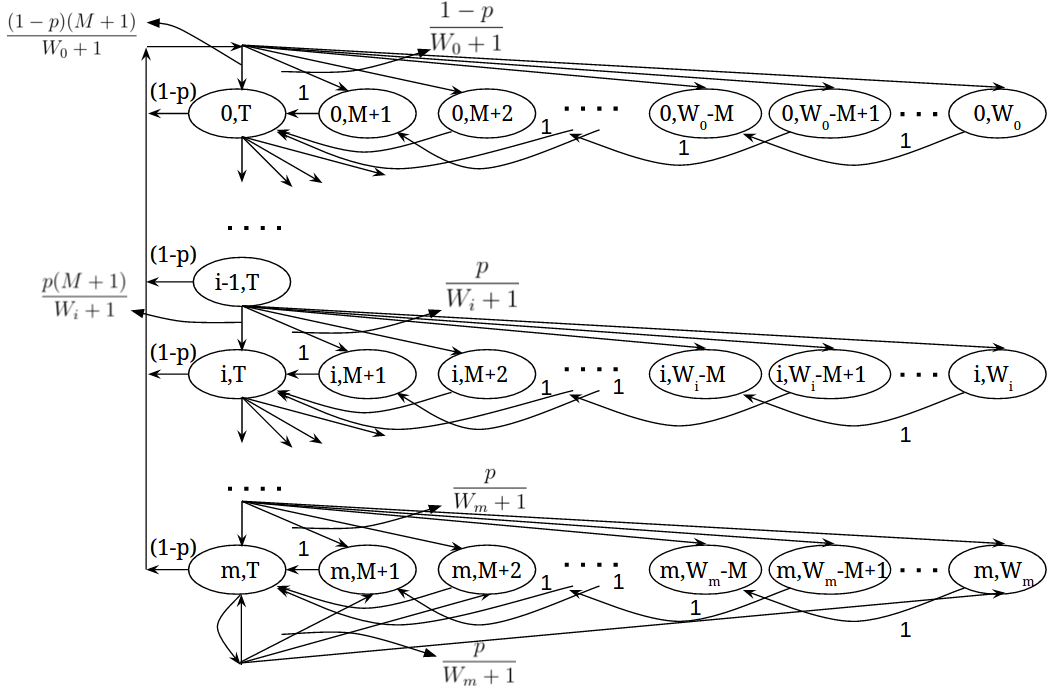
\includegraphics[scale=.45]{./figure/Markov_chain.png}
\caption{Markov Chain model for the backoff window size}
\label{Markov}
\end{figure*}

Let's assume $P\lbrace i_1, k_1|i_0,k_0\rbrace = P\lbrace s(t+1) = i_1, b(t+1)= k_1|s(t) = i_0, b(t) = k_0\rbrace $. In this Markov Chain, the only non null one-step transition probabilities are 
\begin{align}
\left\lbrace
\begin{array}{lll}
P\lbrace i, T | i, k \rbrace = 1  						& k\in [M+1,2M]			& i \in [0,m]\\ [3pt]
P\lbrace i, k-M | i, k \rbrace = 1  						& k\in [2M+1,W_i]   		& i \in [0,m]\\ [3pt]
P\lbrace 0, k | i, T \rbrace = \frac{1-p}{W_0+1}  		& k\in [M+1,W_0]			& i \in [0,m]\\ [3pt]
P\lbrace 0, T | i, T \rbrace = \frac{(1-p)(M+1)}{W_0+1}  &						& i \in [0,m]\\ [3pt]
P\lbrace i, k | i-1, T \rbrace = \frac{p}{W_i+1} 		& k\in [M+1,W_i] 		& i \in [1,m]\\ [3pt]
P\lbrace i, T | i-1, T \rbrace = \frac{p(M+1)}{W_i+1}    &  						& i \in [1,m]\\ [3pt]
P\lbrace m, k | m, T \rbrace = \frac{p}{W_m+1} 		 	& k\in [M+1,W_m] 		& \\ [3pt]
P\lbrace m, k | m, T \rbrace = \frac{p(M+1)}{W_m+1}
\end{array}
\right.
\label{trans_prob}
\end{align}
The first and second equations in \ref{trans_prob} accounts for the fact that in a trigger frame stage for random access, the backoff counter maintained by stations will decrease the number of RUs for random access. 
The third and fourth equation represents that after a successful contention, stations will reset the contention window size to initial window size and uniformly generate a backoff value among $[0,W_0]$, since $T = [0,M]$, the transition probability to $\lbrace i, T \rbrace$ is $M+1$ times of that to $\lbrace i, k \rbrace$. 
For the fifth and sixth equations, they represents when a failure contention occurs, the contention window size will be doubled. 
The last two equation is situation of failure contention at the maximum backoff level.

Let $b_{i,k} = \lim_{t\rightarrow \infty} P\lbrace s(t) = i, b(t) = k\rbrace,\ i\in [0,m], \ k \in [0,W_i]$ be the stationary distribution of the Markov chain. Then we show the steady state for the Markov Chain.
First,  for $k = T$
\begin{align}
b_{i-1,T}\cdot p = b_{i,T} 		\rightarrow b_{i,T} = p^i b_{0,T}, \quad 0\leq i < m\\
b_{m-1,T}\cdot p = (1-p) b_{m,T}	\rightarrow b_{m,T} = \frac{p^m}{1-p}b_{0,T}.
\label{biT}
\end{align}

Then,
\begin{align}
&b_{i,k} =  \nonumber \\
&
\begin{cases}
(\lfloor \frac{W_0-k}{M} \rfloor+1)\frac{(1-p)}{W_0+1}\sum_{i=0}^m b_{i,T}, \  M+1\leq k\leq W_0,\ i = 0\\[3pt]
(\lfloor \frac{W_i-k}{M} \rfloor+1)\frac{p}{W_i+1}b_{i-1,T}, 				\	 M+1 \leq k\leq W_i, \ 0<i<m \\[3pt]
(\lfloor \frac{W_m-k}{M} \rfloor+1)\frac{p}{W_m+1} (b_{m-1,T}+b_{m,T}), 	
\end{cases}\nonumber
\\ &\qquad \qquad \qquad \qquad \quad \qquad \qquad M+1 \leq k\leq W_m, \quad i = m \nonumber \\
\label{steady_prob}
\end{align}

From equation \ref{biT}, we have $\sum_{i=0}^m b_{i,T}= \frac{b_{0,T}}{1-p}$; sum the equation \ref{steady_prob} respectively, we obtain equation \ref{part_sum}.  
\begin{figure*}[!b]
\begin{align}
\begin{cases}
\sum_{k=M+1}^{W_0} b_{0,k} = \frac{b_{0,T}}{W_0+1}\left(-\frac{M}{2}\left\lfloor \frac{W_0}{M}\right\rfloor ^2 + \left(W_0-\frac{M}{2}\right)\left\lfloor \frac{W_0}{M} \right\rfloor \right) \\[8pt]
\sum_{i=1}^{m-1}\sum_{k=M+1}^{W_i} b_{i,k} = \frac{b_{0,T}}{W_0+1}\left(\frac{p}{2}\right)^i \left(-\frac{M}{2}\left\lfloor \frac{W_i}{M}\right\rfloor ^2 + \left(W_i-\frac{M}{2}\right)\left\lfloor \frac{W_i}{M} \right\rfloor \right) \\[8pt]
\sum_{k=M+1}^{W_m} b_{m,k} = \frac{b_{0,T}}{W_0+1}\frac{(\frac{p}{2})^m}{1-p}\left(-\frac{M}{2}\left\lfloor \frac{W_m}{M}\right\rfloor ^2 + \left(W_m-\frac{M}{2}\right)\left\lfloor \frac{W_m}{M} \right\rfloor \right) 
\end{cases}
\label{part_sum}
\end{align}
\end{figure*}

Let $X_i = -\frac{M}{2}\left\lfloor \frac{W_i}{M}\right\rfloor ^2 + \left(W_i-\frac{M}{2}\right)\left\lfloor \frac{W_i}{M} \right\rfloor$. Then we sum all the states to have equation \ref{total_sum2}.
\begin{figure*}[!b]
\begin{align}
1 &= \sum_{i=0}^m \sum_{k=0}^{W_i}b_{i,k} 
 = \frac{b_{0,T}}{W_0+1}\left( X_0 + \sum_{i=1}^{m-1}X_i\left( \frac{p}{2}\right)^i + X_m\frac{\left( \frac{p}{2}\right)^m}{1-p}\right) + \frac{b_{0,T}}{1-p}\label{total_sum}\\
& = b_{0,T}\left( \frac{(1-p)X_0+(1-p) \sum_{i=1}^{m-1}X_i\left( \frac{p}{2}\right)^i+X_m\left( \frac{p}{2}\right)^m+W_0+1}{(W_0+1)(1-p)}\right)\label{total_sum2}
\end{align}
\end{figure*}

We can now express $\tau$, the probability of a station transmit a request at a randomly selected stage.

\begin{align}
\label{tau_general}
&\tau = \sum_{i=0}^m b_{i,T} = \frac{b_{0,T}}{1-p} = \nonumber \\
&\frac{W_0+1}{W_0+1+(1-p)X_0+(1-p) \sum_{i=1}^{m-1}X_i\left( \frac{p}{2}\right)^i+X_m\left( \frac{p}{2}\right)^m}
\end{align}

For $m=0$, check equation \ref{total_sum}, the terms containing $X_i, i>0$ will disappear, and $b_{0,T}/(1-p)$ will just be $b_{0,T}$.
Thus, equation \ref{total_sum2} will be simplified to 
\begin{align}
1 = b_{0,T}\left( \frac{W_0+1+X_0}{W_0+1}\right),
\end{align}
thereby, 
\begin{align}
\tau = b_{0,T} = \frac{W_0+1}{W_0+1+X_0}.
\label{tau_W0}
\end{align}
Thus $\tau$ is independent with $n$, number of contending stations.

On the other hand, conditional collision probability $p$ is the probability that no other stations select the same RU to transmit request. So we have 
\begin{align}
\label{p_ax}
p = 1-\left( 1-\frac{\tau}{M} \right)^{n-1}.
\end{align}
Rewrite the equation \ref{p_ax}, $\tau^\star = \left(1-(1-p)^\frac{1}{n-1} \right)M$. 
To obtain transmission probability $\tau$ and conditional probability $p$, we need to find solutions to group of equations \ref{tau_general} and \ref{p_ax}.
$\tau^\star(p)$ is a monotonically increasing function. 
Though $\tau(p)$ is hard to determine the monotonicity from the expression of equation \ref{tau_general} with respect to $p$. 
We justify the monotonic decrease of function \ref{tau_general} with numerical method. 
Also, $\tau(0) = \frac{W_0+1}{W_0+1+X_0}> \tau^\star(0) = 0$.
And $\tau(1) < \tau^\star(1) = M$. We find the only solution with numerical method.



\section{Random Access Efficiency}
With the transmit probability, we could easily estimate efficiency of random access mechanism. 
Firstly, find expected number of stations who succeed in contending to transmit request at a stage, which is denoted with $E[n_s]$. 
Extending $n_s$, we define a system efficiency as an important metric.
Secondly, we are interested in the access delay of request frame. 
In another word, say how many stages needed for a station to succeed in contending, denoted by $N_{s\_station}$.
What's more, another interesting metric is how many stages are elapsed until a successful stage, which means at least one station succeed in contending in the stage. This metric is a concept similar to "delay" in the second use case of OFDMA-based random access. We represent it with $N_{s\_stage}$. It helps design whole MU UL transmission procedure. 
Here, our concern is mainly on first two metrics which are purely related to random access procedure. The third metric is only expressed in the subsection of access delay, not being discussed later. 

\subsection{$n_s$ and System Efficiency}
What we care in the random access is that how many stations contend successfully in a single stage, denoted by $n_s$.
Given transmission probability $\tau$ and conditional collision probability $p$, we could obtain probability that a station succeeds in contending in a stage, $P_{s\_station} = \tau (1-p)$.
Then, with equation \ref{p_ax}, $E[n_s]$ is easily computed as follows. 
\begin{align}
\label{equ_ns}
E[n_s] &= n P_{s\_station} \nonumber \\
		&= n\tau (1-p) \nonumber \\
		&= n\tau (1-\frac{\tau}{M})^{n-1}
\end{align}

Furthermore, normalizing $n_s$, system efficiency here is defined as 
\begin{align}
\label{eff_def}
\textit{eff}\ (\tau) &= \frac{E[\text{number of successful stations in a given stage}]}{\text{number of RUs for random access in a stgae}} \nonumber\\
					 &=\frac{E[n_s]}{M} \nonumber \\
					 &= \frac{n\tau(1-\frac{\tau}{M})^{n-1}}{M}.
\end{align}

Both two metrics are our concerns. Another metric, access delay, is derived in next subsection.
With all these metrics, we could evaluate the performance later.

	
\subsection{Access Delay}
$N_{s\_station}$, the random variable of how many stages are needed for a station to succeed in contending in a stage follows geometric distribution with parameter $P_{s\_station}$, which is obtained just now.  
Then the expected value of access delay of request frame, $E[D]$, is 
\begin{align}
\label{equ_delay}
E[D] = E[N_{s\_station}] = \frac{1}{\tau (1-\frac{\tau}{M})^{n-1}}.
\end{align}

Then another interesting metric which is not our focus, denoted by $N_{s\_stage}$, that how many stages are elapsed until a successful stage. 
We could firstly obtain $P_{s\_stage}$, the probability of a successful stage, which means at least one station succeed in contending in the stage.

\begin{align}
P_{s\_stage} &= 1-P\lbrace n_s = 0\rbrace \nonumber \\
	&= 1-(1-P_{s\_station})^n \nonumber\\
	&= 1-(1-\tau(1-p))^n
\end{align} 	 
Since $N_{s\_stage}$ follows geometric distribution with parameter $P_{s\_stage}$,  
\begin{align}
E[N_{s\_stage}] &= \frac{1}{P_{s\_stage}}  \nonumber \\
			&= \frac{1}{1-(1-\tau(1-p))^n}
\end{align} 

In a word, we focus on three metrics: number of successful stations in a stage by $n_s$, system efficiency by $E[n_s]/M$ and access delay given by $N_{s\_station}$. 
Actually, only two variables are concerned, $n_s$ and $N_{s\_station}$. However, $n_s$ and its normalized value are both meaningful, which we will explain in following sections.


\section{Model Validation} 		\label{sec_model_val}
To validate the Markov chain model, we run a simulation using C language according to the settings of 802.11ax random access illustration. 
We run the simulation with variety of parameter sets $\lbrace M, m, OCW_{min}\rbrace$ and collects the information of the two variables, $n_s$ and $N_{s\_station}$. 
The validation is given in both figure \ref{validation} and table \ref{table_val}. 
The results show that the Markov model precisely predict the behavior of the OFDMA-based random access.
\begin{table}[!h]
\caption{Analysis versus simulation: $n_s$ and access delay with $m=3,M=9,OCW_{min} = 15$}
\label{table_val}
\begin{center}
\begin{tabular}{c|c|c}
\hline
$n_s$ 	& analysis 	& simulation \\
\hline
$n=1$ 	& 0.72727  	& 0.72728 \\
$n=5$ 	& 2.23001	& 2.22335 \\
$n=10$	& 2.88954	& 2.88546 \\
$n=20$	& 3.29798	& 3.29857 \\
\hline
delay	& analysis	& simulation \\
\hline
$n=1$ 	& 1.37500  	& 1.37499 \\
$n=5$ 	& 2.24214	& 2.24886 \\
$n=10$	& 3.46075	& 3.46565 \\
$n=20$	& 6.06432	& 6.06323 \\
\hline
\end{tabular}
\end{center}
\end{table}

\begin{figure}[!h]
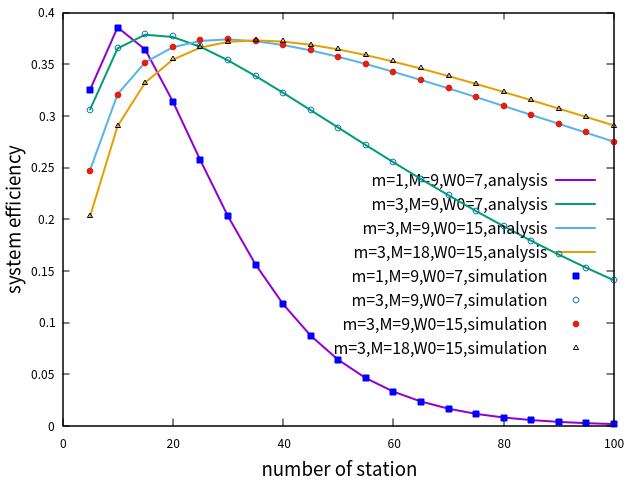
\includegraphics[scale=0.54]{./figure/multiple_parameter.png}
\caption{System efficiency: Analysis versus Simulation}
\label{validation}
\end{figure}
\chapter{Performance Evaluation} \label{chp_perf_eval}
\section{Maximum System Efficiency and Minimum Access Delay} 	\label{sec_max_min}
With the system efficiency given in equation \ref{eff_def}, we take the derivative with respect to $\tau$, and find the extreme point, $\tau^\star = M/n$. Since $\tau\in [0,1]$, $\tau^\star = min\lbrace 1,M/n\rbrace$. 
What we care is when $n$, the number of contending stations, is large, i.e., $\tau^\star = M/n$. 
Then the system efficiency is
\begin{align}
\textit{eff}\ (\tau^\star) = (1-\frac{1}{n})^{n-1} 
\label{equ_max_eff}
\end{align}
Then the maximum $n_s$ is easy to generate.
\begin{align}
\label{equ_max_ns}
E[n_s]^\star = M \cdot \textit{eff}\ (\tau^\star) = M(1-\frac{1}{n})^{n-1} 
\end{align}
Thus the limit of system efficiency, based on infinite $n$, is
\begin{align}
\label{eff_limit}
\lim_{n\rightarrow \infty}\textit{eff}\ (\tau^\star) = \lim_{n\rightarrow \infty}(1-\frac{1}{n})^{n-1} =\frac{1}{e} 
\end{align}

\begin{figure}[!ht]
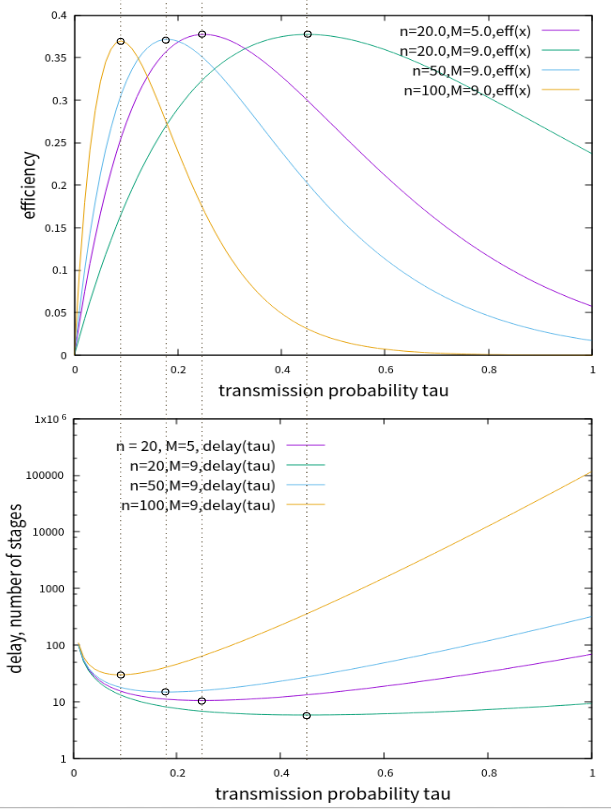
\includegraphics[scale=0.64]{./figure/chp4/max_min.png}
\caption{Efficiency and access delay versus transmission probability $\tau$}
\label{fig_eff_def}
\end{figure}


With the delay analysis given in \ref{equ_delay}, we also take the derivative with respect to $\tau$, and find the extreme point, $\tau^\star = M/n$. Again, $\tau^\star = min\lbrace 1, M/n\rbrace$. 
When $n\geq M$, the minimum access delay is 
\begin{align}
\label{equ_min_delay}
D(\tau^\star) = \frac{n}{M(1-\frac{1}{n})^{n-1}}.
\end{align}

From above analysis, we find that the maximum system efficiency and minimum access delay are both obtained by the same transmission probability $\tau^\star = min\lbrace 1, M/n\rbrace$.
What's more, system efficiency is independent with $M$, number of RUs for random access in a stage, while $M$ affects access delay. 
The larger $M$ is, the shorter the access delay will be. 
It indicates that when AP allocates RUs for random access, the AP could allocates as many as possible, only if the channel of the RU is sensed idle. 
This rule will be more explained in next section.

Figure \ref{fig_eff_def} is plotted corresponding to equation \ref{eff_def} and \ref{equ_delay}.
Consistent to the analysis above, the figure shows that the maximum system efficiency is independent of number of RUs for random access when $n\geq M$, and approaching to $1/e$ with $n$ increasing. 
What's more, the optimal transmission probability $\tau$ of system efficiency and access delay is consistent with each other, which also validates the analysis. 

According to equation \ref{tau_general} and \ref{p_ax}, transmission probability $\tau$ is dependent on system parameters, $M$ (RUs for random access in a stage), $W_0$ (initial contention window) $m$ (backoff levels) or $W_m$ (the maximum contention window) and $n$ (number of stations in the network).
The only way to approach optimal performance is to employ adaptive techniques to tune the system parameter set $\lbrace M, W_0, W_m \rbrace$ on the basis of the estimated value of $n$.
In the following section, we will evaluate the performance corresponding to different system parameters sets and propose the rules to tune the system parameter sets so that the transmission probability $\tau$ approach the optimal transmission probability, $\tau^\star$, which means both system efficiency and delay approach the optimal. 

\section{Rules of Parameter Configuration} 	\label{sec_perf_eval}
We have estimated the maximum system efficiency and minimum access delay in the previous section. Then we evaluate the metrics, $n_s$ (number of stations who succeed in contending in a stage), system efficiency and $D$ (access delay), under various parameter sets. 
With above analysis, we could evaluates transmission probability under various parameter sets, since the optimal transmission probability $\tau^\star$ means both maximum system efficiency and minimal access delay.

At last, we propose rules for configuring the parameter set $\lbrace M, OCW_{min}, OCW_{max}\rbrace$.

\subsection{RUs for Random Access $M$}
\label{M}
Equation \ref{equ_max_eff} indicates that $M$, the number of RUs for random access, has nothing to do with maximum system efficiency. 
However, larger $M$ is better for $n_s$ and $D$ according to equation \ref{equ_max_ns} and \ref{equ_min_delay}. More explaination are given later to validate the statement. 

In figure \ref{fig_n_M_eff}, the maximum system efficiency is the same. 
The difference is "when" the optimal point will be. 
For larger $M$, the optimal number of stations is larger, given by $M/n$. It is also intuitive.

\begin{figure}[!h]
\centering
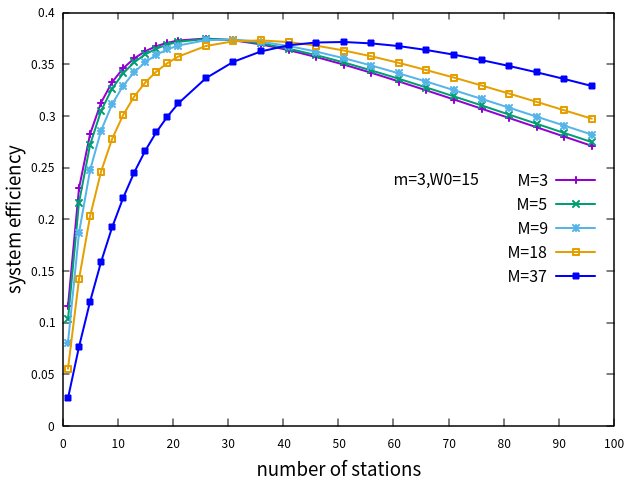
\includegraphics[scale=.85]{./figure/n_M_eff_perf.png}
\caption{System efficiency versus number of stations}
\label{fig_n_M_eff}
\end{figure}

\begin{figure}[!h]
\begin{subfigure}{\textwidth}  
\centering
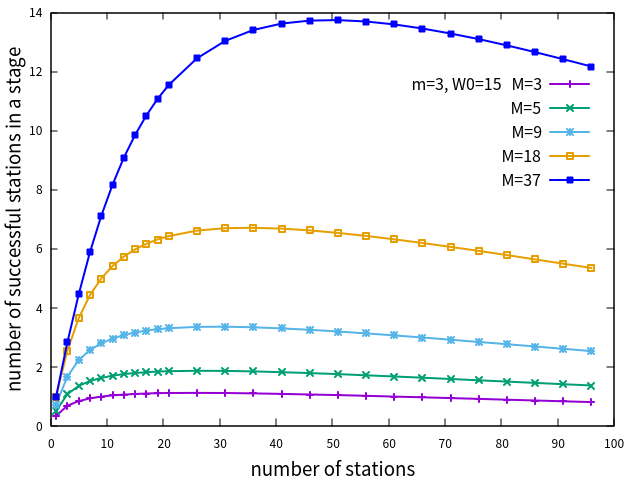
\includegraphics[scale=.85]{./figure/n_M_ns_perf.png}
\caption{Number of successful stations in a single stage versus number of stations}
\label{fig_n_M_ns}
\end{subfigure}

\begin{subfigure}{\textwidth}  
\centering
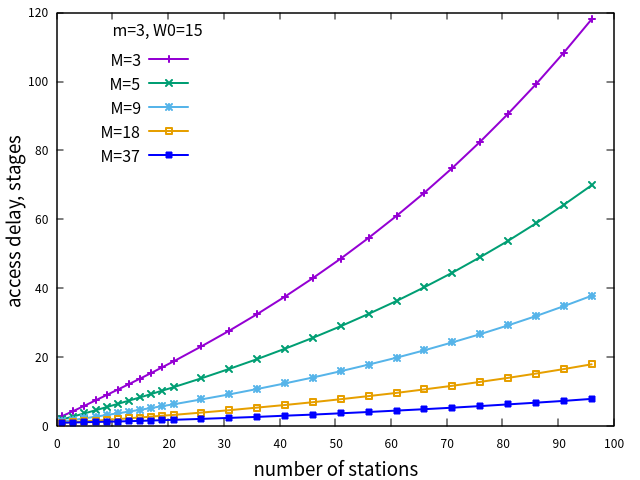
\includegraphics[scale=.85]{./figure/n_M_delay_perf.png}
\caption{Access delay versus number of stations}
\label{fig_n_M_delay}
\end{subfigure}
\caption{Configure $M$}
\end{figure}

In figure \ref{fig_n_M_delay}, the larger $M$ will linearly decrease the access delay of station. The figure is consistent with the equation \ref{equ_min_delay}. 

More practically, we present the number of successful stations in a single stage versus number of stations in figure \ref{fig_n_M_ns}.
While the maximum system efficiency is the same with different $M$, the actually number of stations who succeed contending in a single stage is much different, which corresponds to equation \ref{equ_max_ns}. 
The optimal value of number of successful stations in a single stage is propotional to $M$. 
Above all, when AP allocates RUs for random access, the AP will sense channels first then allocates as many RUs, which are sensed idle, for random access as possible.



\subsection{Initial and max Contention Window $(OCW_{min}, OCW_{max})$}
\label{contend_window}
Different from legacy 802.11 where backoff mechanism is preconfigured in hardware of stations, the initial and maximum contention window $(OCW_{min}, OCW_{max})$ are allocated in beacon frame sent by AP. 
Thus, the configuration of backoff mechanism becomes dynamic, which means that it could be configured according to the scenario, especially the number of stations.
With the $M$ being determined as large as possible, it is more complicated algorithm to adaptive tune $OCW_{min}, OCW_{max}$ so that transmission probability approaches optimal value.
Since $\tau$ is determined by solving equations \ref{tau_general} and \ref{p_ax}, it is hard to give a expression of $\tau$ determined by system parameters $W_0$ and $W_m$.
However, we could find the rules by checking a variety of parameter sets.

% figures
\begin{figure}[!t]
\centering
%subfigure
\begin{subfigure}{\textwidth}
\centering
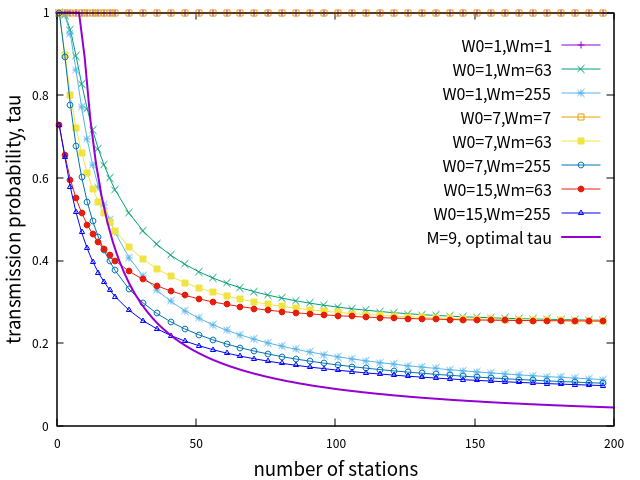
\includegraphics[scale=.85]{./figure/chp4/M9/n_tau_perf_M9_x200.png}
\caption{Case 1, given $M=9$}
\label{fig_tau_n_M9}
\end{subfigure}
%subfigure
\begin{subfigure}{\textwidth}
\centering
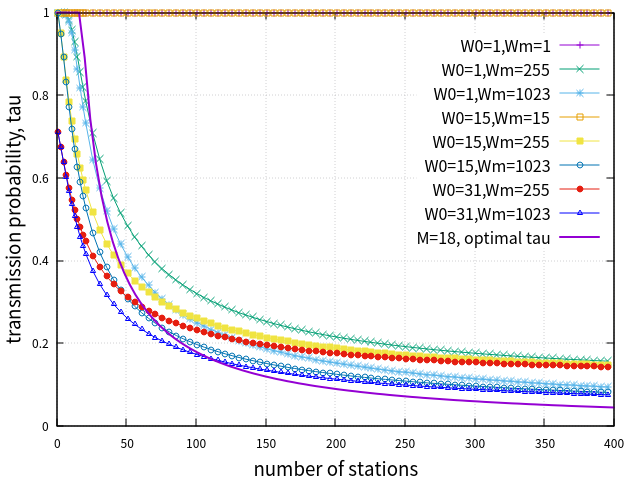
\includegraphics[scale=.85]{./figure/chp4/M18/n_tau_perf_M18_x400.png}
\caption{Case 1, given $M=18$}
\label{fig_tau_n_M18}
\end{subfigure}
%caption
\caption{Transmission probability versus number of stations}
\label{fig_tau_n}
\end{figure}

Figure \ref{fig_tau_n} shows case 1 ($M=9$) and case 2 ($M=18$), from both of which we could generalize some rules between $\tau$ and parameters $OCW_{min}, OCW_{max}$.
In the figure, the purple line without point is the optimal $\tau$, which is given according to $\tau^\star = min\lbrace 1, M/n \rbrace$.
As stated above, we need to find a tuning of $OCW_{min}, OCW_{max}$ so that $\tau$ approaches the optimal line. The rules are listed following.

Firstly, the $OCW_{min}$, namely $W_0$, determines the start of the line of $\tau$. The larger $W_0$ is, the lower transmission probability will start at $n=1$.
A special situation is when $W_0<M$, $\tau=1$ at $n=1$. 
That's why cases in figure \ref{fig_tau_n} have two different start points.
For optimal transmission probability $\tau^\star$, when $n \leq M$, $\tau^\star = 1$. 
A special case of $m=0$, which means $W_m=W_0$, results in constant transmission probability equal to 1, which is perfect match with $\tau^\star$ at $n\leq M$.
Thus, if given $n\leq M$, the optimal configuration will be $OCW_{max}= OCW_{min} < M$. 


Secondly, $W_m$ determines limit of the $\tau$, i.e., where the line will converge. 
Lines with the same $W_m$ will converge to a same value. 
To see the tendency of lines, I draw the two figures \ref{fig_tau_n_M9} and \ref{fig_tau_n_M18} with $n$ in range $[0,200]$ and $[0,400]$ respectively. 
And both the two figures validate the above statement.
And larger $W_m$ is closer to optimal transmission probability when $n$ is large. 
When $m=0$, $\tau$ will not change with $n$, which is consistent with equation \ref{tau_W0}.
For those $m>0$, the curve will be convex. It is intuitive that with the number of stations increasing, the collision probability will increase, thus contention window increase. 


% figures
\begin{figure}[!t]
\centering
\begin{subfigure}{\textwidth}
\centering
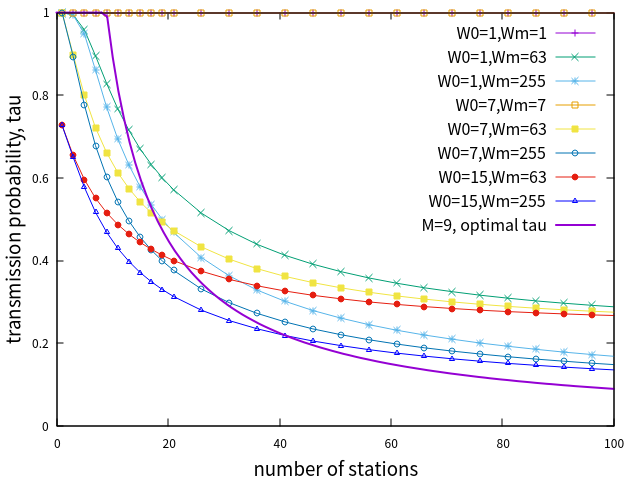
\includegraphics[scale=.85]{./figure/chp4/M9/n_tau_perf_M9_x100.png}
\caption{Case 1, given $M=9$}
\label{fig_tau_n_M9_detail}
\end{subfigure}

\begin{subfigure}{\textwidth}
\centering
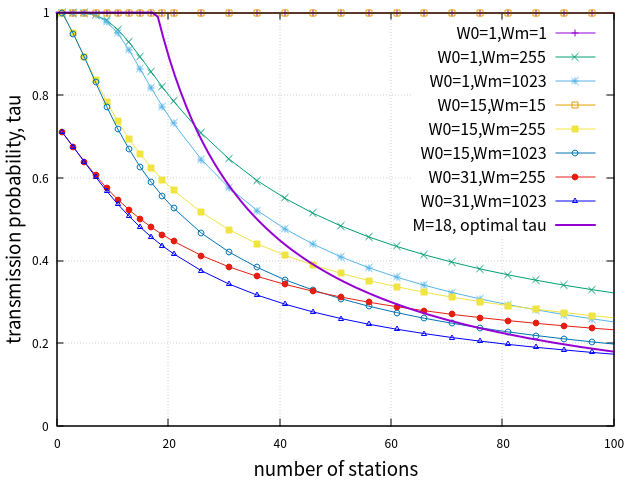
\includegraphics[scale=.85]{./figure/chp4/M18/n_tau_perf_M18_x100.png}
\caption{Case 1, given $M=18$}
\label{fig_tau_n_M18_detail}
\end{subfigure}

\caption{Details of transmission probability versus number of stations when $n\leq 100$}
\label{fig_tau_n_detail}
\end{figure}

Then, we draw two figures with x axis range $[0,100]$ to find more rules as in figure \ref{fig_tau_n_detail}. 
From the two figures \ref{fig_tau_n_M9_detail} and \ref{fig_tau_n_M18_detail} we find another rule that if $W_0=1$ which is the minimum value, there will be a flat start of $\tau$.
What's good is that the flat start is closer to $\tau^\star$ when $n\leq M$.

Based on above observation, we find conclude that $W_0$ has significant influence on small $n\leq M$, while $W_m$ affects $n$ is large or $n>M$. 
Afterwards, in the next two subsections, we check the system efficiency and access delay under different parameter sets of $\lbrace W_0, W_m \rbrace$, with which we could find explicit relationship between the parameter and performance.




\subsubsection{Configure $OCW_{max}$}

\begin{figure}[!t]
\centering
\begin{subfigure}{\textwidth}  
  \centering  
  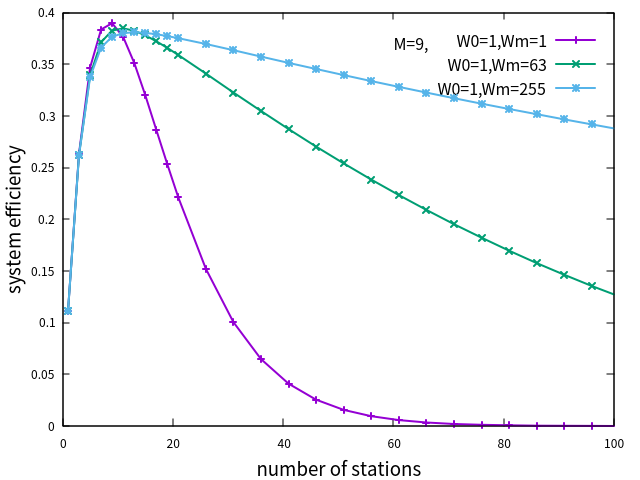
\includegraphics[scale=0.85]{./figure/chp4/M9/n_eff_perf_W01.png}  
    \caption{System efficiency versus number of stations}   
    \label{fig_n_eff_Wm}
\end{subfigure}   

\begin{subfigure}{\textwidth}
	\centering
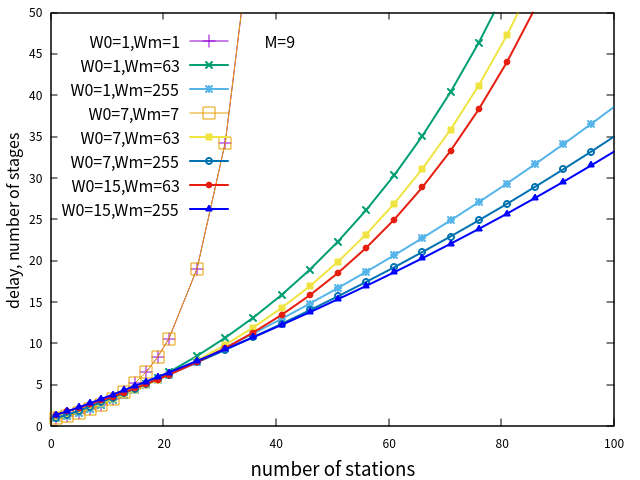
\includegraphics[scale=.85]{./figure/chp4/M9/n_delay_perf.png}
\caption{Access delay versus number of stations}
\label{fig_n_delay_Wm}
\end{subfigure}
\caption{Example of Configuring $OCW_{max}$, given $M=9$}
\end{figure}

With above rough rules, we estimate the effects of $OCW_{max}$ first by setting different $OCW_{max}$ while given $OCW_{min}=1$ and $M=9$.
It is because small $OCW_{min}$ is good for situation of small $n$.
Actually the data we use to generate the figures are the same as that for figure \ref{fig_tau_n_M9}. For figure \ref{fig_n_eff_Wm}, we display three of them to clearly show relationship between system efficiency and $OCW_{max}$.
And from the figure, it is apparent that larger $OCW_{max}$ is better for system efficiency. 
The result corresponds to the second rule we obtain when estimating the transmission probability $\tau$.
What's more, the access delay also validates the same result. And since we use the same data with that in figure \ref{fig_tau_n_M9}, we find that the lines which converge in figure \ref{fig_tau_n_M9} also have the same tendency in figure \ref{fig_n_delay_Wm}. 

As stated in last section that $OCW_{max}$ has significant influence on situation of large $n$, $n$ is number of contending stations. With increasing $n$, larger $OCW_{max}$ will obtain larger gain. 
Therefore, we have a rule that the larger $OCW_{max}$, the better.



\subsubsection{Configure $OCW_{min}$}

\begin{figure}[!t]
\centering
\begin{subfigure}{\textwidth}  
  \centering  
  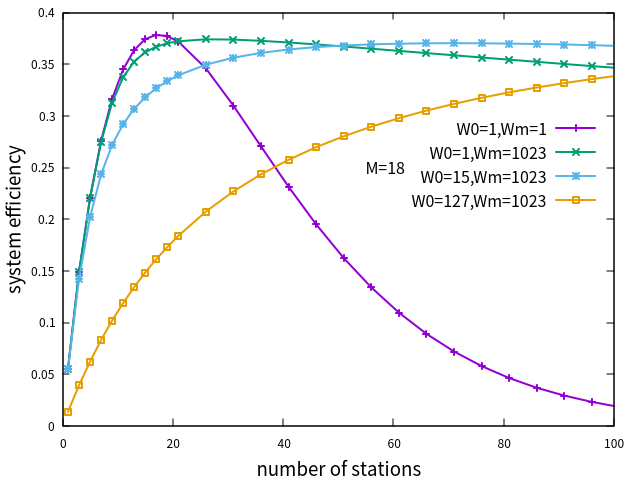
\includegraphics[scale=0.85]{./figure/chp4/M18/n_eff_perf_Wm1023.png}  
    \caption{System efficiency versus number of stations}   
    \label{fig_n_eff_W0}
\end{subfigure}   

\begin{subfigure}{\textwidth}
	\centering
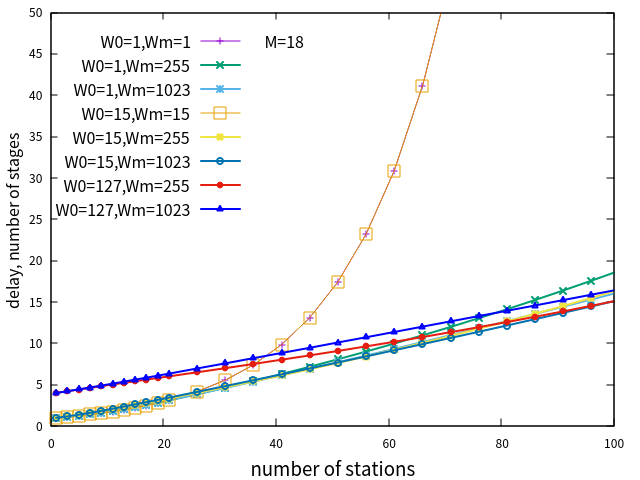
\includegraphics[scale=.85]{./figure/chp4/M18/n_delay_perf.png}
\caption{Access delay versus number of stations}
\label{fig_n_delay_W0}
\end{subfigure}
\caption{Example of Configuring $OCW_{min}$, given $M=18$}
\end{figure}

Similarly, to estimate the relationship between performance and $OCW_{min}$, we compare the performance between different $OCW_{min}$ while given fixed $OCW_{max}=1023$, which has been validated that large $OCW_{max}$ is better, and $M=18$. 
Firstly, we claimed in section \ref{contend_window} that $W_0=W_m\leq M$ is the perfect configuration in situation of $n\leq M$. It is again validated here that it has the maximum system efficiency and minimum access delay in situation of $n\leq M$. 
Secondly, since $OCW_{min}$ determines the start of line, i.e., $n=1$, it has significant influence on small $n$.
From figure \ref{fig_n_eff_W0} and \ref{fig_n_delay_W0}, we find larger $OCW_{min}=127$ has lower system efficiency and longer access delay. And as stated before, $W_0=15$ has close performance with $W_0=1$ since $W_0<M$ will be similar for situation of small $n$.

Therefore, we generate a rule that the smaller $OCW_{min}$, the better.
For a special situation that $n\leq M$, we could configure $OCW_{min}=OCW_{max}<M$, which will result in perfect performance. 
However, larger $OCW_{max}$ smaller $OCW_{min}$ is closely approach to optimal performance.

\subsection{Rules for configuring $\lbrace M, OCW_{min}, OCW_{max} \rbrace$}
Above two previous subsections, we could conclude rules of configuring the parameter set $\lbrace M, OCW_{min}, OCW_{max} \rbrace$ for obtaining best performance for all $n$. 
\begin{itemize}
\item[Rule 1] Large $M$
\item[Rule 2] $OCW_{min}, OCW_{max}$
	\begin{itemize}
	\item small $OCW_{min}$ and large $OCW_{max}$
	\item If given $n\leq M$
	\begin{itemize}
		\item $OCW_{max}=OCW_{min}<M$
	\end{itemize}
	\end{itemize}
\end{itemize}

%After we propose the rules of configuring the parameter set $\lbrace M, OCW_{min}, OCW_{max} \rbrace$, we run another analysis with typical group parameter sets which validate our rules.

%From figure \ref{fig_n_ns_val}, larger $M = 18$  results in larger $n_s$, number of successful stations in a single stage, than $M=9$. Thus, $M$ is as large as possible.
%Then given a $M=18$ as an example, smaller $W_0 = 7$ and larger $m = 7$ have better performance than other parameter sets when $n>M$.
%
%For the system state that $n\leq M$, $n_s$ and access delay of $m=0,W_0 = 7$ is the best case among all the parameter sets. It is because the transmission probability under such condition reaches the optimal value as in figure \ref{fig_n_tau}.  

%\begin{figure}[!ht]
%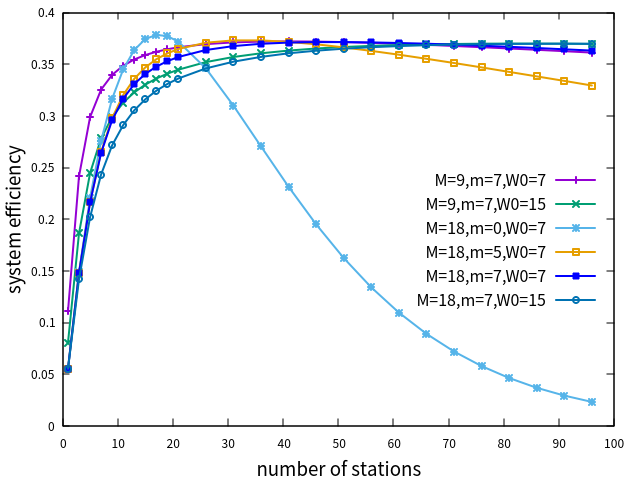
\includegraphics[scale=.54]{./figure/n_rule_eff_perf.png}
%\caption{System efficiency versus number of stations}
%\label{fig_n_eff_val}
%\end{figure}
%
%\begin{figure}[!ht]
%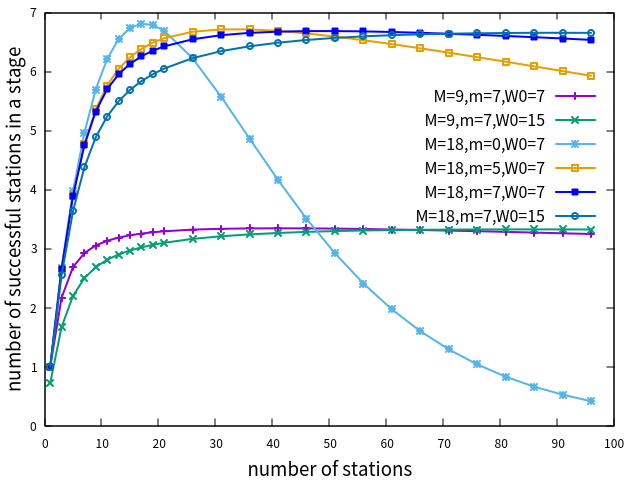
\includegraphics[scale=.54]{./figure/n_rule_ns_perf.png}
%\caption{$n_s$ versus number of stations}
%\label{fig_n_ns_val}
%\end{figure}
%
%\begin{figure}[!ht]
%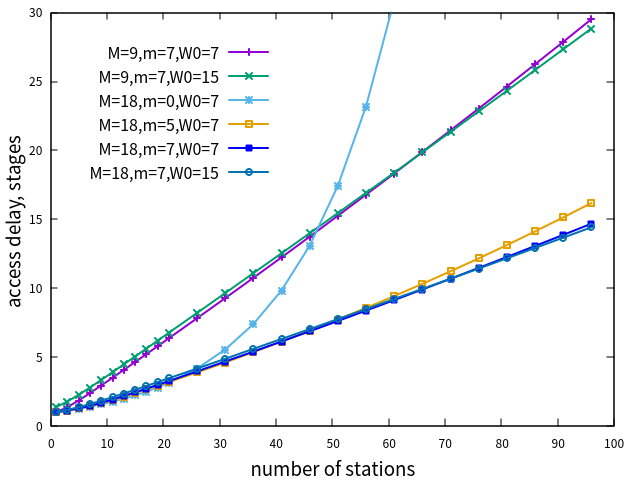
\includegraphics[scale=.54]{./figure/n_rule_delay_perf.png}
%\caption{Access Delay versus number of stations}
%\label{fig_n_delay_val}
%\end{figure}

\chapter{Conclusion}   \label{chp_conclu}
In this thesis, we first expose that the bottleneck of legacy 802.11 is located at its MAC, instability of DCF and unfair queueing problem. 
Then we introduce 802.11ax as a solution which aimed at high efficient WLAN (HEW).
One of the important features of 802.11ax is OFDMA-based random access, which is MU random access in IEEE 802.11ax MAC. 
The system parameters are configured by AP dynamically, so it is more flexible and more complicated. 

Afterwards, we extend Bianchi's Markov chain model of DCF to model the OFDMA-based random access for its simplicity and accuracy. 
With the model we do saturation analysis to depict the steady state behavior of the mechanism.
Simulation validates the model. 
Then we could estimate the impact of a parameter set $\lbrace M, OCW_{min}, OCW_{max} \rbrace$ on system efficiency and access delay, where $M$ is the number of RUs for random access,  and $OCW_{min}, OCW_{max}$ is the initial and maximum OFDMA contention window. 
At last, rules of configuration of the parameter set aimed at approaching the optimal transmission probability $\tau^\star$ is proposed for AP with or without given number of contending stations.
%\input{related}
%\input{photoshoot}
%\input{modeling}
%\input{application}
%\input{conclusion}

\appendix

\backmatter

\addcontentsline{toc}{chapter}{\bibname}
\bibliographystyle{abbrv}

% Your bibliography goes here
\bibliography{thesis}

\end{document}
